%%%%%%%%%%%%%%%%%%%%%%%%%%%%%%%%%%%%%%%%%%%%%%%%%%%%%%%%%%%%%%%%%%%%%%%%%%%%%%%%
% Introduction
%%%%%%%%%%%%%%%%%%%%%%%%%%%%%%%%%%%%%%%%%%%%%%%%%%%%%%%%%%%%%%%%%%%%%%%%%%%%%%%%
\subsection{Introduction}
\label{hls:introduction}
\nocite{Xilinx:Tutorial}
\gls{HLS} is a process of converting a program that was written in a
higher-level language (such as \progLang{C}, \progLang{C++} or
\progLang{SystemC}) into an \gls{RTL} implementation for use with an \gls{FPGA}.
In particular, the \gls{HLS} tool \software{AutoESL} was used for this
\thesis{}. When synthesising an \gls{RTL} implementation, there are two
competing design goals that could be targeted. The first is to create a design
with the smallest area; the second is a design with the highest throughput. Each
design goal may have a bit emphasis depending on the nature of the application.

The key advantage of \gls{HLS} tools is that development time for a high-level
programming language is much smaller than development time for a \gls{RTL}
\gls{HDL} programming language \cite{Berkeley:2010}. In addition, programming in
an \gls{RTL} \gls{HDL} programming language is much more error prone and
requires a vastly different skill set. The main criteria that must be considered
when choosing to use a \gls{HLS} tool for hardware development is whether use of
the tool deliver substantial improvements in productivity without compromising
the performance and efficiency of the hardware design.

In \software{AutoESL}, the design flow for \gls{HLS} involves the following
stages \cite{Xilinx:Tutorial}:
\begin{enumerate}
    \item \textbf{Elaboration:} Elaborates the source code into an internal
        database containing operators. The operators represent operations in the
        \progLang{C} code such as additions, multiplications, array reads and
        writes. See \autoref{hls:operators}.
    \item \textbf{Synthesis:} Maps the operators to cores from the
        \software{AutoESL} library. Cores are the specific hardware components
        used to create the design (such as adders, multipliers, pipelined
        multipliers and block \glspl{RAM}). See \autoref{hls:cores}.
    \begin{enumerate}
        \item \textbf{Scheduling:} Scheduling determines in which cycles
            operations can occur.
        \item \textbf{Binding:} Scheduled operations are bound to specific
            hardware implementations.
    \end{enumerate}
    \item \textbf{Simulation:} Verifies the \gls{RTL} through co-simulation with
        the \progLang{C} test bench.
    \item \textbf{Implementation:} Generates and executes the scripts to perform
        logic synthesis.
\end{enumerate}

\begin{figure}
    \centering
    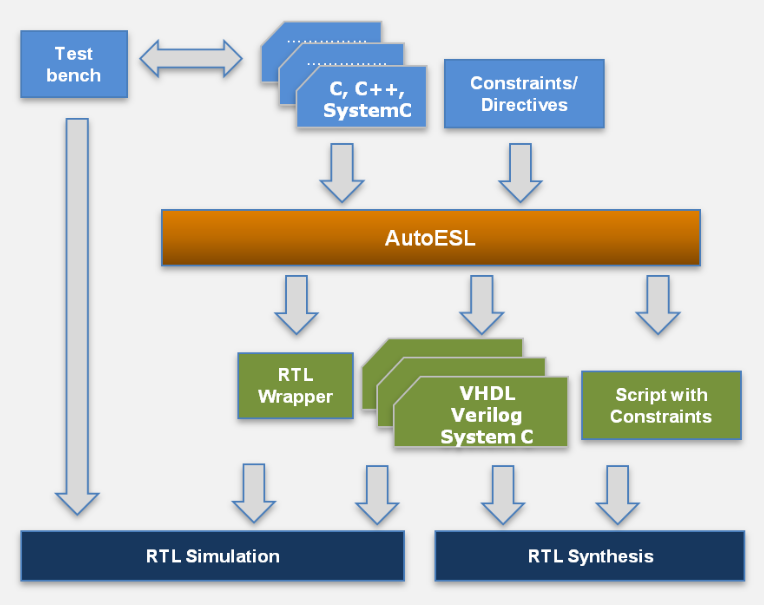
\includegraphics[width=0.8\textwidth]{xilinx/autoesl-use-case}
    \caption{AutoESL use case}
    \label{fig:autoesl:useCase}
\end{figure}

The synthesis process handles a single top level function from the higher-level
language source code as the basis for the \gls{RTL} implementation. The
arguments to this top level functions are synthesised into \gls{RTL} ports
through a process known as interface synthesis \cite{Xilinx:CodingStyleGuide}.
Interface synthesis automatically handles the data sequencing to and from the
design: the user simply needs to select the appropriate interface. Many types of
interfaces can be synthesized: wire ports, single and two-way handshakes, RAM
access ports and FIFO ports among others.

\begin{figure}
    \centering
    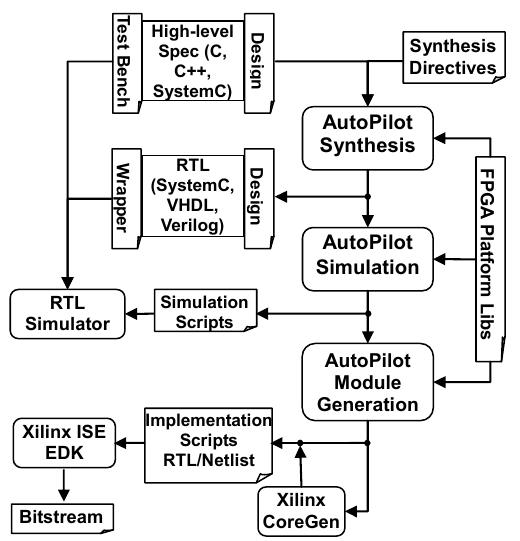
\includegraphics[width=0.8\textwidth]{xilinx/xilinx-flow}
    \caption{Xilinx flow}
    \label{fig:xilinx:flow}
\end{figure}

From an \software{AutoESL} synthesised design, Xilinx's \gls{RTL} tools (namely
\gls{ISE} and \gls{EDK}) allow the \gls{RTL} design to be transformed into a
complete \gls{FPGA} design in the form of a bitstream. The Xilinx \gls{HLS}
tools also generate wrappers that allow for the \gls{FPGA} design to be
interfaced with external memory and \gls{IO} resources.